\documentclass[a4paper,10pt,notitlepage,pdftex,headsepline]{scrartcl}

\usepackage{a4wide}
\usepackage{cmap} % чтобы работал поиск по PDF
\usepackage[utf8]{inputenc}
\usepackage[russian]{babel}
\usepackage[T2A]{fontenc}

\usepackage{textcase}
\usepackage[pdftex]{graphicx}

\pdfcompresslevel=9 % сжимать PDF
\usepackage{pdflscape} % для возможности альбомного размещения некоторых страниц
\usepackage[pdftex]{hyperref}
% настройка ссылок в оглавлении для pdf формата
\hypersetup{unicode=true,
            pdftitle={РГР по ВС},
            pdfauthor={Погода Михаил},
            pdfcreator={pdflatex},
            pdfsubject={},
            pdfborder    = {0 0 0},
            bookmarksopen,
            bookmarksnumbered,
            bookmarksopenlevel = 2,
            pdfkeywords={},
            colorlinks=true, % установка цвета ссылок в оглавлении
            citecolor=black,
            filecolor=black,
            linkcolor=black,
            urlcolor=blue}

\usepackage{amsmath}
\usepackage{amssymb}
\usepackage{moreverb}
%for \includepdf
%\usepackage{pdfpages}

\author{Михаил Погода}
\title{Расчётно-графическая работа по вычислительным системам}
\date{\today}
\begin{document}
\maketitle

\section{Условие}

\begin{figure}[h]
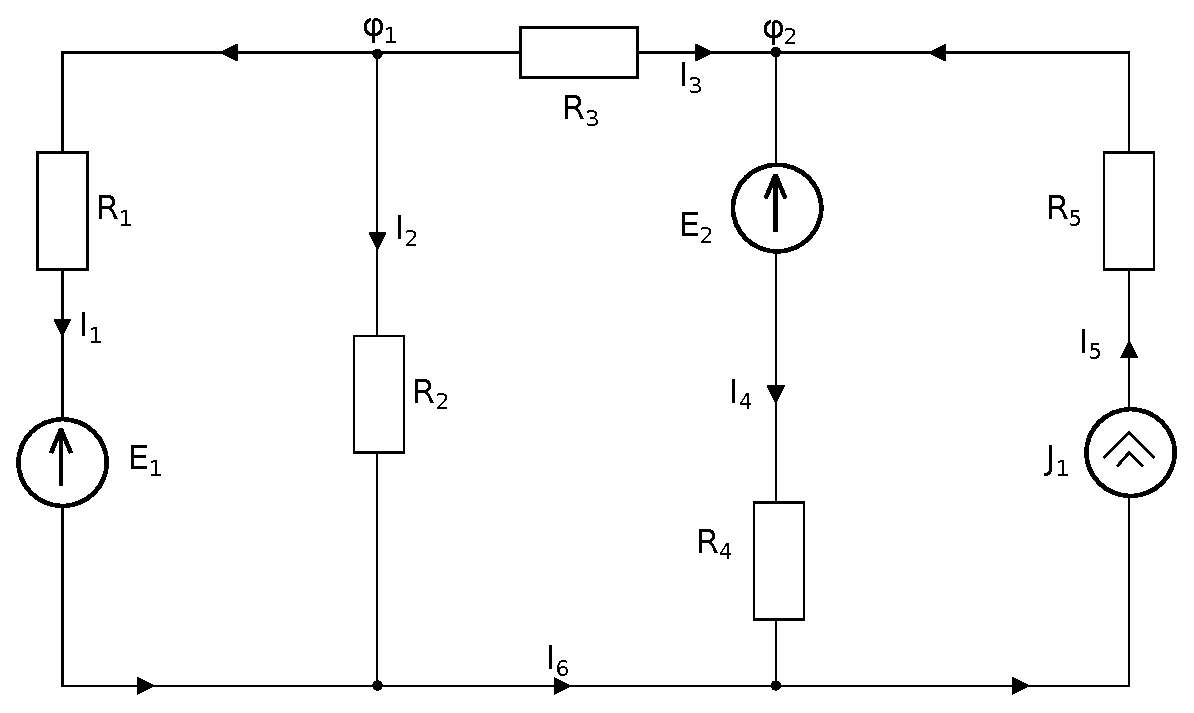
\includegraphics[scale=0.75]{schema.eps}
\caption{Вариант 11}
\end{figure}

\begin{tabular}{cc}
$R_1$ & $20$ Ом\\
$R_2$ & $30$ Ом\\
$R_3$ & $10$ Ом\\
$R_4$ & $50$ Ом\\
$R_5$ & $10$ Ом\\
$E_1$ & $40$ В\\
$E_2$ & $20$ В\\
$J_1$ & $5$ А
\end{tabular}

\section{Выбор метода}
Воспользуемся \textit{методом узловых потенциалов}.

Введём потенциалы узлов схемы $\varphi_1$, $\varphi_2$ для первого и второго узлов соответственно.

\section{Система уравнений по первому закону Кирхгоффа}
$$
\begin{cases}
-I_1 - I_2 - I_3 = 0, & \text{в узле} \varphi_1\\
I_3 - I_4 + I_5 = 0, & \text{в узле} \varphi_2
\end{cases}
$$
\section{Применяем закон Ома и переходим от потенциалов к напряжению между узлами}
$$
\begin{cases}
-\frac{\varphi_1-E_1}{R_1} - \frac{\varphi_1}{R_2} - \frac{\varphi_1-\varphi_2}{R_3} = 0\\
\frac{\varphi_1-\varphi_2}{R_3} - \frac{\varphi_2-E_2}{R_4}+J_1 = 0
\end{cases}
$$
\section{Преобразуем уравнения к стандартному виду}
$$
\begin{cases}
\varphi_1 \left( \frac{1}{R_1} + \frac{1}{R_2} + \frac{1}{R_3} \right) - \frac{\varphi_2}{R_3} = \frac{E_1}{R_1}\\
\varphi_1 \left( -\frac{1}{R_3} \right) + \varphi_2 \left( \frac{1}{R_3} + \frac{1}{R_4} \right) = \frac{E_2}{R_4} + J_1
\end{cases}
$$
\section{Найдём потенциалы}
$$
\left( \begin{matrix}
\frac{1}{20} + \frac{1}{30} + \frac{1}{10} & -\frac{1}{10} \\ 
-\frac{1}{10} & \frac{1}{10} + \frac{1}{50}
\end{matrix} \right)
\left( \begin{matrix}
\varphi_1\\
\varphi_2\\
\end{matrix} \right)
=
\left( \begin{matrix}
\frac{40}{20}\\
\frac{20}{50} + 5
\end{matrix} \right)
$$

\begin{tabular}{cc}
$\varphi_1$ & $65$ В\\
$\varphi_2$ & $99.167$ В\\
$\varphi_3$ & $0$ В\\
$\varphi_4$ & $0$ В
\end{tabular}

\section{Найдём токи, протекающие через резисторы}
$$I_1 = \frac{\varphi_1 - \varphi_3 - E_1}{R_1} = 1.25 \text{А}$$
$$I_2 = \frac{\varphi_1 - \varphi_3}{R_2} = 2.1667 \text{А}$$
$$I_3 = \frac{\varphi_1 - \varphi_2}{R_3} = -3.4167 \text{А}$$
$$I_4 = \frac{\varphi_3 - \varphi_4}{R_4} = 1.5833 \text{А}$$
$$I_5 = J_1 = 5 \text{А}$$

Отрицательное значение $I_3$ говорит о том, что мы выбрали неправильное направление тока $I_3$.

\section{Проверим энергетический баланс}

$$\sum\limits_{k=1}^5 I_k^2 R_k = \sum\limits_{k=1}^2 E_k I_k + U_1 J_1$$

$$\sum\limits_{k=1}^5 I_k^2 R_k = 31.25 + 140.833 + 116.736 + 125.347 + 250 = 664.167 \text{Вт}$$
$$\sum\limits_{k=1}^2 E_k I_k = -50 - 31.6667 = -81.6667 \text{Вт}$$
$$U_1 J_1 = \left(\varphi_2 - \varphi_4 + I_5 R_5\right) J_1 = \left( 99.167 + 50 \right) \cdot 5 = 745.835 \text{Вт}$$

$$\frac{\left|664.167-664.1683\right|}{664.167} \cdot 100\% = 0.0002\%$$

Т.\,к. погрешность мала, можно считать, что баланс сошёлся.


\end{document}